% -*- coding: utf-8 -*-

\chapter{Hardware utilizado}\label{ap:hardware}
Aunque ya se han introducido algunas descripciones del hardware empleado, a continuación se añade algo más de información sobre sus características.

\section{Plataforma móvil B21r}
La plataforma más usada en los experimentos del proyecto corresponde al modelo B21r de la empresa iRobot. Se trata de una plataforma holonómica cuyo sistema motriz es de tipo synchro-drive con cuatro ruedas directrices y motrices. Los sensores de infrarrojos y de ultrasonidos que posee no se han utilizado por su menor precisión, fiabilidad y rango respecto al escáner láser LMS200 (sección \ref{laser}).

\begin{figure}[h]
  % Requires \usepackage{graphicx}
  \centering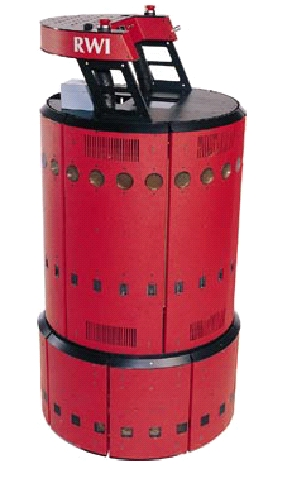
\includegraphics[scale=0.4]{b21r}\\
  \caption{Plataforma móvil B21r de iRobot}\label{fg:b21r}
\end{figure}

En la parte superior del robot hay dos pulsadores rojos que sirven para activar los frenos del robot en caso necesario. Pueden quitarse pulsando nuevamente alguno de estos botones o a través del panel de control del robot girando el botón negro situado junto a él.
\clearpage
Las principales características de este robot se presentan en la siguiente tabla:
\begin{table}[h]
\begin{center}
\begin{tabular}{|l|c|} \hline
Característica & B21r\\
\hline
\hline
Diámetro & 52cm\\
\hline
Altura & 106cm\\
\hline
Distancia al suelo & 2.54cm\\
\hline
Peso & 122.5kg\\
\hline
Capacidad de carga & 90kg\\
\hline
Baterías & 4x12V estancas plomo-ácido\\
\hline
\hline
Autonomía & 6 h\\
\hline
Sistema Motriz & Synchro-drive 4 ruedas\\
\hline
Motores & 4 servomotores 24V\\
\hline
Ruedas & Goma maciza\\
\hline
\hline
Diámetro ruedas & 11cm\\
\hline
Ancho ruedas & 3cm\\
\hline
Sistema de giro & Synchro-drive 4 ruedas\\
\hline
Radio máxima curvatura & 0cm\\
\hline
Radio giro & 0cm (robot holonómico)\\
\hline
\hline
Máxima velocidad avance & 0.9m/seg.\\
\hline
Máxima velocidad de giro & 167º/seg.\\
\hline
Terreno & Interiores planos y uniformes\\
\hline
Resolución avance & 1mm\\
\hline
Resolución giro & 0.35º\\
\hline
\end{tabular}
\end{center}
\caption{Características del robot B21r de iRobot}
\end{table}

El robot tiene un PC base con Red Hat Linux. También dispone de un PC secundario con sistema operativo Windows. El acceso de bajo nivel al hardware del robot lo llevan a cabo unos programas servidores incluidos en el software proporcionado por iRobot (denominado \emph{Mobility} y basado en el estándar de programación distribuida CORBA). El único de estos servidores que se ha utilizado es el b21server (alias base), encargado del manejo de los motores y de la obtención de medidas de los sensores.

\section{Plataforma móvil Pioneer P3-AT de MobileRobots/ActivMedia Robotics}
Este robot no ha podido ser utilizado en la mayor parte de las pruebas por no disponer de sensor láser para detectar obstáculos, construir mapas y situarse correctamente en su entorno de operación. Sin embargo, la utilización del sistema implementado será prácticamente inmediata tan pronto como se tenga un láser instalado.

Se trata de una plataforma utilizable en todo tipo de terrenos (AT son las siglas de \emph{All Terrain}) También permite un alto grado de carga.Posee tracción a las cuatro ruedas y la realización de giros se basa en el deslizamiento. Esto repercute en la estimación de la odometría, resultando ser bastante peor que la proporcionada por el B21r.

\begin{figure}[h]
  % Requires \usepackage{graphicx}
  \centering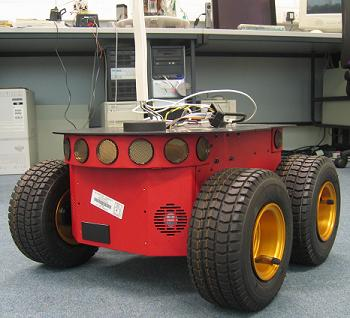
\includegraphics[scale=0.4]{P3AT}\\
  \caption{Plataforma móvil Pioneer P3-AT}\label{fg:P3AT}
\end{figure}

El cuerpo del robot es de aluminio y su parte delantera se puede desmontar con facilidad por medio de unos tornillos. En la plataforma superior del robot está situado el panel de control, que permite acceder al microcontrolador y dispone de algunos LEDs indicadores de estado. En él también se haya el puerto serie RS-232 utilizado para establecer la conexión con el equipo en el que se ejecuta el software de control desarrollado.

\begin{figure}[h]
  % Requires \usepackage{graphicx}
  \centering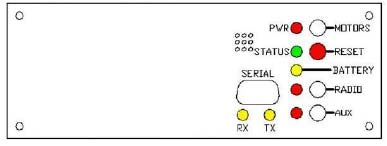
\includegraphics[scale=0.5]{panel}\\
  \caption{Panel de control}\label{fg:panel}
\end{figure}

A continuación se resumen en una tabla las principales características de este robot:
\begin{table}[h]
\begin{center}
\begin{tabular}{|l|c|} \hline
Característica & Pioneer P3-AT\\
\hline
\hline
Largo & 50cm\\
\hline
Ancho & 49cm\\
\hline
Alto & 26cm\\
\hline
Distancia al suelo & 8cm\\
\hline
Peso & 12kg\\
\hline
Carga útil & 32kg\\
\hline
Cuerpo & 1.6mm aluminio pintado h\\
\hline
Baterías & 12V estanca, plomo-ácido\\
\hline
\hline
Autonomía & 4-8 h\\
\hline
Sistema Motriz & 4 ruedas motrices\\
\hline
Ruedas &  Neumáticas nylon\\
\hline
\hline
Diámetro ruedas & 21.5cm\\
\hline
Ancho ruedas & 8.8cm\\
\hline
Sistema de giro & Deslizamiento diferencial\\
\hline
Radio máxima curvatura & 40cm\\
\hline
Radio giro & 0cm\\
\hline
\hline
Máxima velocidad avance & 1.2m/seg.\\
\hline
Máximo escalón & 10cm\\
\hline
Máximo hueco & 15.2cm\\
\hline
Máxima pendiente & 40\\
\hline
Terreno & Asfalto, tierra, césped, etc.\\
\hline
Encoders & 500pulsos\\
\hline
Procesador & Hitachi H8S\\
\hline
\end{tabular}
\end{center}
\caption{Características del robot Pioneer P3-AT de MobileRobots}
\end{table}



\clearpage
\section{Escáner láser LMS200}\label{laser}
Este escáner láser se ha utilizado como único sensor estereoceptivo debido a sus elevadas prestaciones en comparación con las de los sensores de infrarrojos y ultrasonidos. Se encuentra instalado en la parte superior del robot Urbano (a 1.2m de altura), desplazado 16.8cm hacia delante con respecto al centro de la plataforma B21r. El fabricante es la empresa alemana SICK.

\begin{figure}[h]
  % Requires \usepackage{graphicx}
  \centering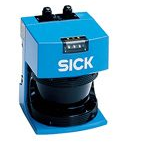
\includegraphics[scale=0.6]{laser}\\
  \caption{Láser LMS200 de SICK}\label{fg:laser}
\end{figure}

Utiliza un haz láser infrarrojo de clase I (inofensivo para el ojo humano incluso en tiempos de exposición prolongados) para la obtención de medidas de distancia con gran precisión y rapidez. El barrido es de 180º y las medidas tomadas son prácticamente independientes de la reflectancia de los objetos.

Presenta varias opciones de funcionamiento que permiten variar el alcance, la precisión y el número de medidas en cada barrido del láser.

La siguiente tabla contiene sus principales características:

\begin{table}[h]
\begin{center}
\begin{tabular}{|l|c|} \hline
Característica & LMS-200\\
\hline
\hline
Resolución angular & 1º/0.5º/0.25º\\
\hline
Tiempo de respuesta & 13ms/26ms/53ms\\
\hline
Resolución & 10mm\\
\hline
Error sistemático (modo mm) & $\pm$15mm\\
\hline
Error estadístico (1 Sigma) & 5mm\\
\hline
Clase láser & 1 (eye-safe)\\
\hline
\hline
Máxima distancia & 80m\\
\hline
Interfase de datos & RS422/RS232\\
\hline
Velocidad transferencia & 9.6/19.2/38.4/500 kBaud\\
\hline
Alimentación & 24V DC $\pm$ 15\%\\
\hline
\hline
Consumo & 20 W\\
\hline
Peso & 4.5kg\\
\hline
Ancho & 155mm\\
\hline
Alto & 210mm\\
\hline
Profundo & 156mm\\
\hline
\end{tabular}
\end{center}
\caption{Características del láser SICK LMS-200}
\end{table}



